\documentclass[a4paper, 12pt]{extarticle}

%%% Includes 
\usepackage[utf8]{inputenc} % UTF-8 encode 
\usepackage[english, russian]{babel}
\usepackage{geometry} % adjust page layout 
\usepackage{graphicx} 
\usepackage{hyperref} 
\usepackage{amsmath} % math formulas 
\usepackage{amsthm} % theorems, definitions, etc.
\usepackage{setspace} % for set line spacing 
\usepackage{indentfirst} % indent on a first line after the paragraph 
% \usepackage{pgfplots} % for plots 
\usepackage{listings} % for code listings 
\usepackage{xcolor} % colors (used for listings)
\usepackage{sourcecodepro} % for another monospaced font 
\usepackage{cmap} % for correct search in pdf
\usepackage{placeins} % for \FloatBarrier
\usepackage{enumitem} % for custom lists


%%% Debug
% \usepackage{showframe} % frame borders for demonstration 


%%% Custom commands
% commands for unnumbered sections
\newcommand{\usection}[1]{\section*{#1} \addcontentsline{toc}{section}{\protect\numberline{}#1}}
\newcommand{\usubsection}[1]{\subsection*{#1} \addcontentsline{toc}{subsection}{\protect\numberline{}#1}}
\newcommand{\usubsubsection}[1]{\subsubsection*{#1} \addcontentsline{toc}{subsubsection}{\protect\numberline{}#1}}

% math commands
\theoremstyle{definition}
\newtheorem{definition}{Определение}

\theoremstyle{plain}
\newtheorem{theorem}{Теорема}
\newtheorem*{thproof}{Доказательство}
\newtheorem*{example}{Пример}

\theoremstyle{remark}
\newtheorem*{notabene}{Замечание}
\newtheorem*{solution}{Решение}


% Redefinition of section and subsection numbering style (with dot at the end)
\def\thesection{\arabic{section}.}
\def\thesubsection{\arabic{section}.\arabic{subsection}.}
\def\thesubsubsection{\arabic{section}.\arabic{subsection}.\arabic{subsubsection}.}

% Theorems, definitions, etc.



%%% Settings for links 
\hypersetup{
    colorlinks,
    citecolor=black,
    filecolor=black,
    linkcolor=black,
    urlcolor=black
}


%%% Layout
\geometry{
	left=17mm, % left margin
	top=17mm, % top margin
	right=17mm, % right margin
	bottom=20mm, % bottom margin
	marginparsep=0mm, % space between text and margin notes
	marginparwidth=0mm, % width of margin notes
	headheight=8mm, % height of the header
	headsep=5mm, % space between header and text
}


\linespread{1.5} % line spacing
\setlength{\parskip}{\baselineskip}  % Add space between paragraphs

\setlist{itemsep=1pt,topsep=1pt,parsep=1pt} % custom list settings


% overfull hbox settings
\tolerance 5000 % default 200, max 10000, 
\hbadness 3000 % default 1000, max 10000, warning threshold for underfull hbox
\emergencystretch 0pt  % default 0pt, how much the lines can stretch for the sake of good line breaks
\hfuzz 0.4pt % ignore overfull box less than 
\widowpenalty=10000 % no lines at the start of the page
\vfuzz \hfuzz % don't care about underfull vbox if overfull is acceptable
\raggedbottom % if the page is not filled, align the content to the bottom


%%% Redefinition of table of contents command to get centered heading
\makeatletter
\renewcommand\tableofcontents{ 
  \begin{singlespace}
    \null\hfill\textbf{\Large\contentsname}\hfill\null\par
    \@mkboth{\MakeUppercase\contentsname}{\MakeUppercase\contentsname}%
    \@starttoc{toc}
  \end{singlespace}
}
\makeatother


%%% Listings settings
\definecolor{codegreen}{rgb}{0, 0.6, 0}
\definecolor{codegray}{rgb}{0.5, 0.5, 0.5}
\definecolor{codepurple}{rgb}{0.58, 0, 0.82}
\definecolor{backcolour_gray}{rgb}{0.98, 0.98, 0.98}

\lstdefinestyle{python_white}{
  language=Python,
  backgroundcolor=\color{backcolour_gray},   
  commentstyle=\color{codegreen},
  keywordstyle=\color{blue},
  numberstyle=\tiny\color{codegray},
  stringstyle=\color{codepurple},
  basicstyle=\ttfamily\small\singlespacing,
  breakatwhitespace=true,         
  breaklines=true,                 
  captionpos=b, % t/b                  
  keepspaces=true,                 
  numbers=none, % none/left/rigth                    
  numbersep=5pt,                  
  showspaces=false,                
  showstringspaces=false,
  showtabs=false,                  
  tabsize=2,
  frame=single, % none/leftline/topline/bottomline/lines/single/shadowbox
  rulecolor=\color{gray}, % frame color 
}

\lstset{style=python_white} % set default listings style



%%% For title page
\def\name{Отчет по лабораторной работе №5} 
\def\subject{По дисциплине "Линейные системы автоматического управления"}
\def\subname{Типовые динамические звенья}
\def\madeby{Александр Иванов, R3338}
\def\teacher{Перегудин А.А.\\ Пашенко А.В.}

\begin{document}

% Title page 
\begin{titlepage}

\thispagestyle{empty}

\title{

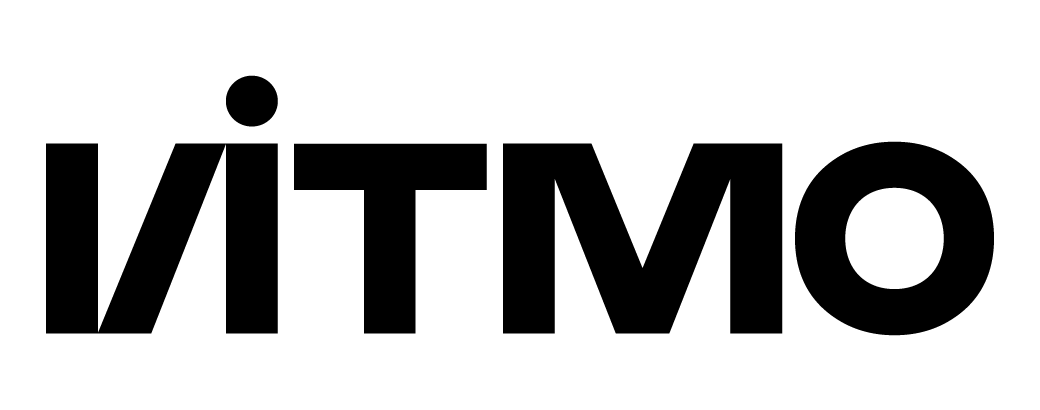
\includegraphics[width=4cm]{media/ITMO_logo.png} 

\vspace{1em}
НИУ ИТМО 
\vspace{4em}

\begin{center}
\Large\textsc{\textbf{\name}}

\normalsize\textsc{\textbf{\subject}}

\vspace{1em}
``\subname'' 

Вариант 30

\end{center}

\vspace{3em}

\begin{flushright}
\normalsize{ 
Выполнил: \\ \textbf{\madeby} 

Преподаватели: \\ \textbf{\teacher} 
}
\end{flushright}	

\vfill

\begin{center}
\small{Санкт-Петербург, \the\year}
\end{center}
}


\author{}
\date{}
\maketitle
\thispagestyle{empty}
\end{titlepage} % Title page

\addtocounter{page}{1} % Inc counter to start from 2 
\tableofcontents % Table of contents
\pagebreak

\section{Исследование управляемости}

Рассмотрим систему $\dot{x} = Ax + Bu$, где 
\begin{equation}
    \begin{array}{cc}
        A = \begin{bmatrix}
            5 & -2 & 8 \\
            4 & -3 & 4 \\
            -4 & 0 & -7
        \end{bmatrix}, &
        B = \begin{bmatrix}
            -7 \\
            -5 \\
            7
        \end{bmatrix}
    \end{array}
\end{equation}

\subsection{Управляемость системы}
\subsubsection{Матрица управляемости}
Найдем матрицу управляемости $U = [B, AB, A^2B]$: 
\begin{equation}
    U = \begin{bmatrix} 
        \begin{array}{c|c|c}
            \begin{bmatrix}
                -7 \\
                -5 \\
                7
            \end{bmatrix} & 
            \begin{bmatrix}
                5 & -2 & 8 \\
                4 & -3 & 4 \\
                -4 & 0 & -7
            \end{bmatrix} \times 
            \begin{bmatrix}
                -7 \\
                -5 \\
                7
            \end{bmatrix} &
            \begin{bmatrix}
                5 & -2 & 8 \\
                4 & -3 & 4 \\
                -4 & 0 & -7
            \end{bmatrix}^2 \times
            \begin{bmatrix}
                -7 \\
                -5 \\
                7
            \end{bmatrix}
        \end{array}   
    \end{bmatrix}
\end{equation}
\begin{equation}
    U = \begin{bmatrix}
        -7 & 31 & -43 \\
        -5 & 15 & -5 \\
        7 & -21 & 23 \\
    \end{bmatrix}
\end{equation}
Определим ранг матрицы управляемости:
\begin{equation}
    \text{rank}(U) = 3
\end{equation}
Так как ранг матрицы управляемости равен порядку системы, то система является полностью управляемой согласно критерию Калмана.

\subsubsection{Управляемость собственных значений}
Найдем спектр матрицы $A$:
\begin{equation}
    \sigma(A) = \{-3, -1-2j, -1+2j\}
\end{equation}

Для каждого собственного значения найдем матрицу Хаутуса $H_i = \begin{bmatrix} A - \lambda_i I & B \end{bmatrix}$ и определим ее ранг:
\begin{enumerate}
    \item $\lambda_1 = -3$: $H_1 = \begin{bmatrix}
        8 & -2 & 8 & -7\\
        4 & 0 & 4 & -5 \\
        -4 & 0 & -4 & 7
    \end{bmatrix}$, $\text{rank}(H_1) = 3$, собственное значение управляемо.
    \item $\lambda_2 = -1-2j$: $H_2 = \begin{bmatrix}
        6+2j & -2 & 8 & -7\\
        4 & -2+2j & 4 & -5 \\
        -4 & 0 & -6+2j & 7
    \end{bmatrix}$, $\text{rank}(H_2) = 3$, собственное значение управляемо.
    \item $\lambda_3 = -1+2j$: $H_3 = \begin{bmatrix}
        6-2j & -2 & 8 & -7\\
        4 & -2-2j & 4 & -5 \\
        -4 & 0 & -6-2j & 7
    \end{bmatrix}$, $\text{rank}(H_3) = 3$, собственное значение управляемо.
\end{enumerate}
Так как выше было показано, что система является полностью управляемой, то каждое собственное значение матрицы $A$ является управляемым. 

\subsubsection{Диагональная форма системы}
Найдем диагональную форму системы, заменив базис на базис из собственных векторов матрицы $A$:
\begin{equation}
    \dot{\hat{x}} = P^{-1}AP\hat{x} + P^{-1}Bu
\end{equation}
Где $P$ -- матрица собственных векторов матрицы $A$. 
Найдем собственные векторы матрицы $A$:
\begin{equation}
    \begin{array}{ccc}
        v_1 = \begin{bmatrix} -1 \\ 0 \\ 1 \end{bmatrix} &
        v_2 = \begin{bmatrix} -3+j \\ -2 \\ 2 \end{bmatrix} &
        v_3 = \begin{bmatrix} -3-j \\ -2 \\ 2 \end{bmatrix} 
    \end{array}
\end{equation}
Тогда матрица $P$:
\begin{equation}
    P = \begin{bmatrix}
        -1 & -3+j & -3-j \\
        0 & -2 & -2 \\
        1 & 2 & 2
    \end{bmatrix}
\end{equation}
Система преобразуется к виду:
\begin{equation}
    \dot{\hat{x}} = \begin{bmatrix}
        -3 & 0 & 0 \\
        0 & -1-2j & 0 \\
        0 & 0 & -1+2j
    \end{bmatrix} \hat{x} + 
    \begin{bmatrix}
        2 \\
        \frac{5 - 5j}{4} \\ 
        \frac{5 + 5j}{4}
    \end{bmatrix} u
\end{equation}
Так как все элементы $P^{-1}B$ не равны нулю, то система является полностью управляемой, каждая мода системы управляема.

\subsection{Грамиан управляемости}
Найдем грамиан управляемости $P(t_1)$:
\begin{equation}
    P(t_1) = \int_{0}^{t_1} e^{At}BB^Te^{A^Tt}dt
\end{equation}
Вычислим грамиан управляемости для $t_1 = 3$ с помощью функции \texttt{gram}: 
\begin{equation}
    P(3) = \begin{bmatrix}
        18.12 & 10.97 & -11.64 \\ 
        10.97 & 7.48 & -8.48 \\ 
        -11.64 & -8.48 & 10.14 \\ 
    \end{bmatrix}
\end{equation}
Найдем собственные числа Грамиана управляемости: 
\begin{equation}
    \sigma(P(3)) = \{ 0.05, 1.94, 33.74 \}
\end{equation}
Все собственные числа Грамиана управляемости положительны, что говорит о том, что система является управляемой.


\subsection{Управление системой}
Найдем управление $u(t)$, которое будет переводить систему из состояния $x(0) = 0$ в состояние $x_1 = x(t_1) = \begin{bmatrix} -2 & -3 & 3 \end{bmatrix}^T$. 
\begin{equation}
    u(t) = B^Te^{A^T(t_1 - t)}P(t_1)^{-1}x_1
\end{equation}
Реализуем данное управление в MATLAB и проведем моделирование системы. 
\begin{figure}
    \centering
    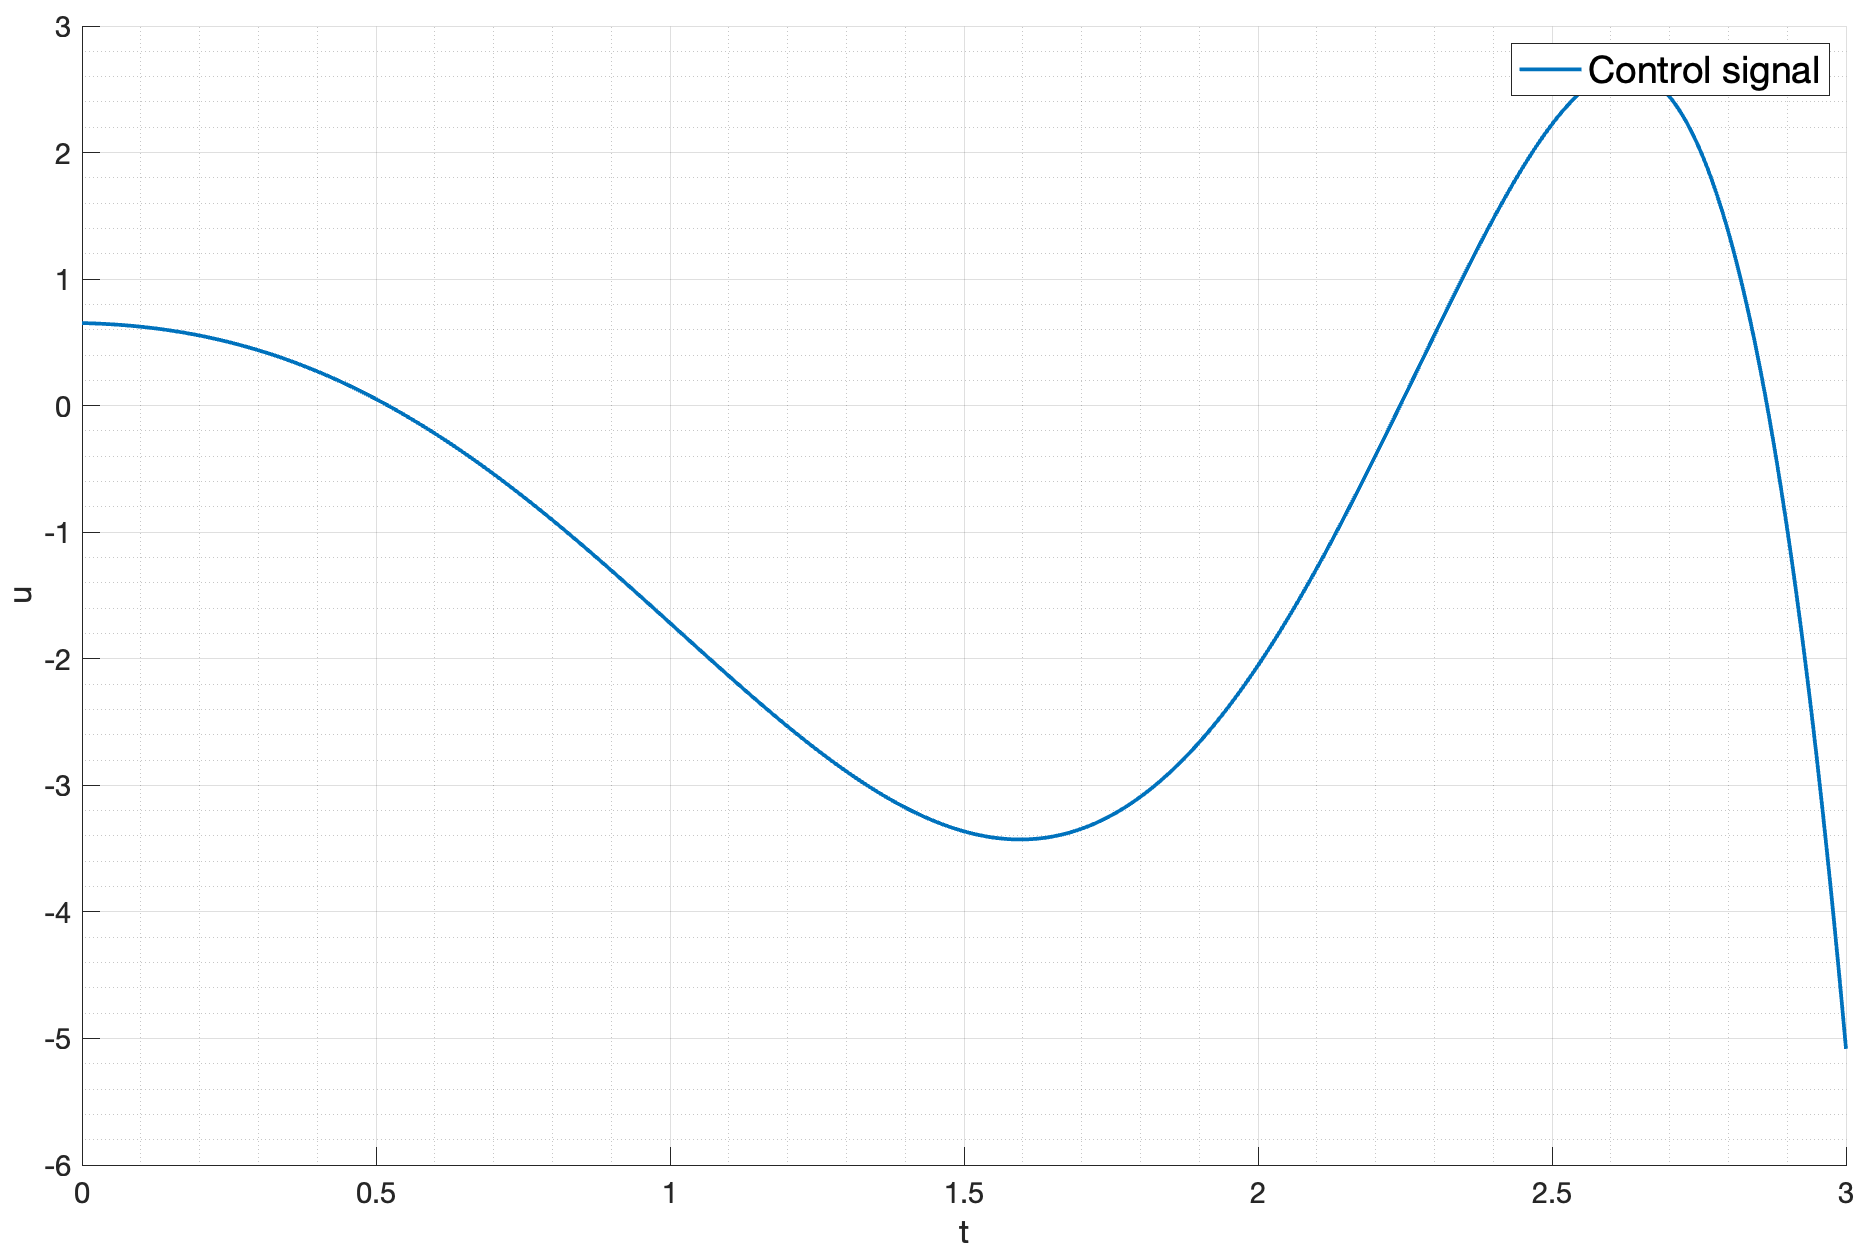
\includegraphics[width=\textwidth]{media/plots/task1_control_signal.png}
    \caption{Управление системой}
    \label{fig:task1_control_signal}
\end{figure}
На рисунке \ref{fig:task1_control_signal} изображено управление системой.
\begin{figure}
    \centering
    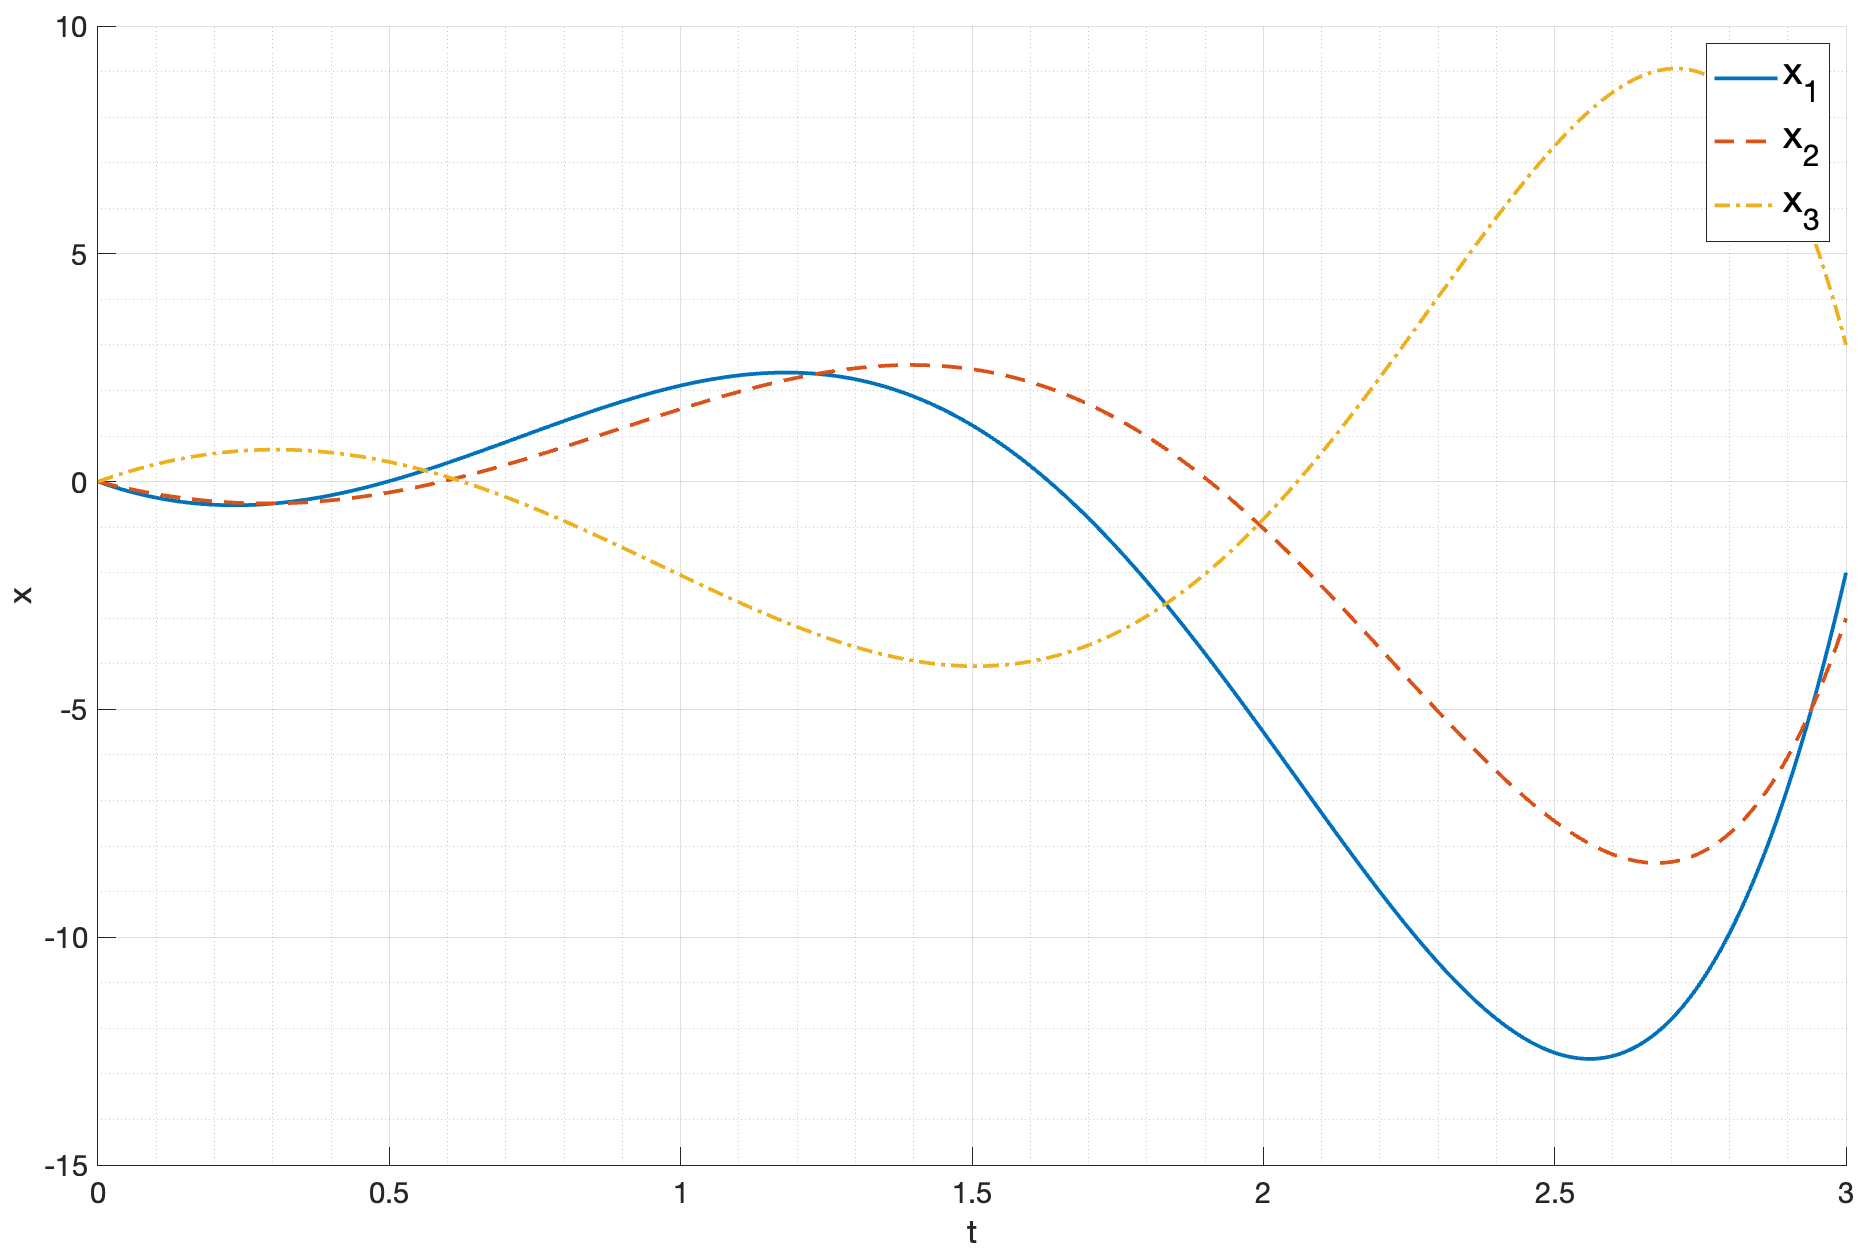
\includegraphics[width=\textwidth]{media/plots/task1_states.png}
    \caption{Состояние системы}
    \label{fig:task1_state}
\end{figure}
На рисунке \ref{fig:task1_state} изображено состояние системы.

Видно, что система управляемая в соответствии с заданным управлением и переходит в заданное состояние. 
\FloatBarrier
\subsection{Вывод}
При исследовании системы, рассматриваемой в этом заднии, удалось показать, что она является 
полностью управляемой. Это было продемонстрировано с помощью критерия Калмана, через 
управляемость собственных значений и диагональную форму системы. Также был найден грамиан 
управляемости и проверены его собственные числа. Проведено моделирование системы с управлением, 
которое переводит систему в заданное состояние. Результаты моделирования показали, что система
управляема и управление работает корректно. 
\FloatBarrier % Content

\end{document}